\subsection{Probing the Deuteron Wavefunction}

It was suggested for some time~\cite{Frankfurt:1981mk} that to resolve the microscopic structure of nuclei one needs to study scattering at sufficiently large momentum transfer and large relative momenta of the produced nucleons. This logic was confirmed~\cite{Arrington:2011xs} by a series of experiments at SLAC~\cite{Frankfurt:1993sp} and JLab~\cite{Arrington:1998ps,Fomin:2011ng} that directly observed short-range correlations (SRC) in a series of nuclei, and established a similar effect of SRC in the deuteron and in heavier nuclei with $pn$ correlations giving the dominant contribution.  Hence, the deuteron serves as a ``hydrogen atom" for the studies of the microscopic short-range structure of the nuclei since it is the simplest nuclei that follows SRC scaling.

To achieve further progress, it is necessary to improve our knowledge of the deuteron wave function at high momenta, and to separate the S and D contributions to the high momentum component of the deuteron. The dominance of the D-wave at large range of the nucleon momenta is expected in a range of the theoretical models as shown in Fig.~\ref{sd-wf}, but experimentally it was probed in a rather indirect way via measurement of $T_{20}$ for the deuteron form factor~\cite{Garcon:2001sz}. Still, the knowledge of S/D ratio for large momenta is rather poor. Indeed, all wavefunctions are constrained by low energy data to reproduce the S/D ratio at small momenta while the overall probability of the D-wave in the deuteron differs by a factor up to 1.5, leading to a large difference of the S/D ratio at large momenta.

The S and D-states are related to the tensor asymmetry $A_{zz}$ by~\cite{Frankfurt:1988nt}
\begin{equation}
	A_{zz} \propto \frac{\frac{1}{2}w^2(k)-u(k)w(k)\sqrt{2}}{u^2(k)+w^2(k)},
\end{equation}
where $u(k)$ is the S-state wave function and $w(k)$ is the D-state wave function. Additionally, measuring $A_{zz}$ at lower $Q^2$ will map out the transition from hadronic to partonic degrees of freedom.

\begin{figure}
\begin{center}
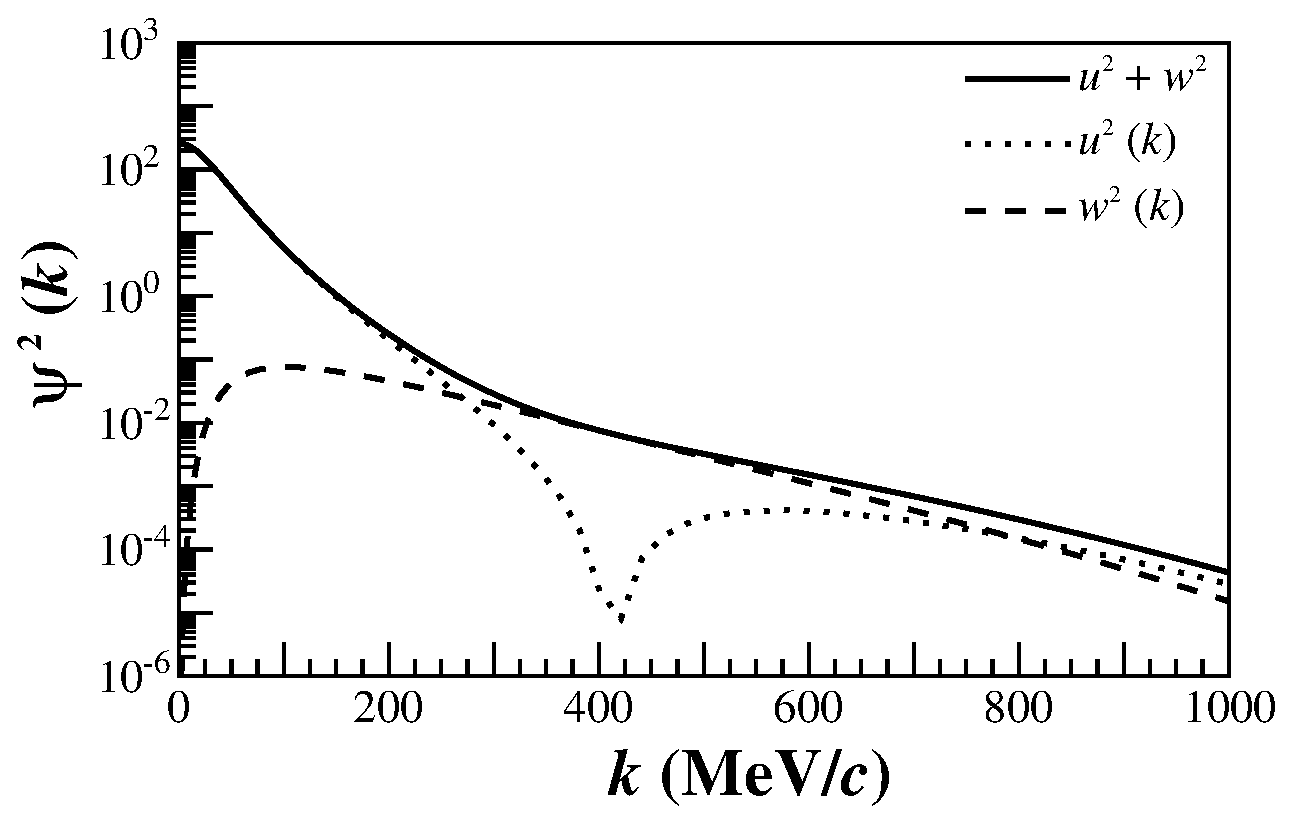
\includegraphics[width=0.55\textwidth]{figs/sd_wf_av18.eps}
\caption{\label{sd-wf} The AV18~\cite{PhysRevC.84.034003} deuteron wave-function, showing the dominance of the D-state (dashed) in comparison to the S-state (dotted) in the full wavefunction (solid) at high momentum ($k>300\mathrm{~Mev}/c$).}
\end{center}
\end{figure}

Ratios of inclusive cross sections at $x>1$ has demonstrated an early onset of the scaling of the ratios when plotted as a function of the light-cone fraction of the struck nucleon momentum.  As a result, the ratios provide a direct measurement of the ratio of the high momentum components in nuclei.  Similarly, one can expect that in the case of scattering from the polarized deuteron we expect the early scaling for the asymmetry when plotted as a function of the minimal struck nucleon momentum or the light cone fraction in the A($e,e’$) case.
It was observed at JLab that the scaling of the ratios is setting in starting at $Q^2 \sim 1 \mathrm{~GeV}^2$ so covering the range of $Q^2$ up to 2~GeV$^2$ will be sufficient to  measure the S/D ratios in an interesting momentum range. 





%For decades~\cite{PhysRev.81.165}, it has been known that the nucleon-nucleon potential has a short-range repulsive core, which is responsible for the stability of strongly interacting matter. However, a description of the repulsive core remains largely unconstrained and our understanding of QCD dynamics at short distances ($\leq 0.5\mathrm{~fm}$) largely incomplete~\cite{Sargsian:2014bwa}. 


It is worth noting here that in addition to comparing predictions for the different wave functions, one expects to be able to distinguish between non-relativistic and light cone quantum mechanic models.  The principal difference between the models is the relation between the spectator momentum and momentum in the wave function in the nonrelativistic model they coincide, while in the light cone model the relation is non-linear starting at $k \sim 250 \mathrm{~MeV}/c$. This difference is most clearly manifested in the scattering off the polarized deuteron due to a strong dependence of the S/D ratio on the nucleon momentum.